\section{Discussion and Future Work}
Though the presented work helps address some of the challenges faced by contemporary behavioral researchers, in some places there remains uncertainty in the meaning of the visualizations and even more deeply hidden discoveries.
Additionally, new scientific questions have been raised through application of these visualizations and thus future work is required.


\subsection{Dealing With Overlapped Data Frames}
When looking at data surrounding an event, we must be cognizant of how instances of the same event at another time may effect our data.
For instance, if our analysis targets the 30m following an event, and the event frequently occurs at 10m intervals, the overlapping signals will create unwanted artifacts.

\begin{figure}
\centering
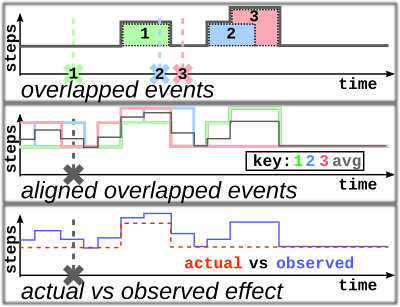
\includegraphics[width=0.6\columnwidth]{./img/eventOverlapExample.png}
\caption{Overlapping analysis windows confounds observed effect after time-alignment.}
\label{fig:overlapExample}
\end{figure}

Figure \ref{fig:overlapExample} illustrates this point by showing how events falling within each other's windows of analysis confound the data and ultimately yields a signal quite unlike the actual effect response.
In real data, this is further complicated by the non-linear way in which effects are expected to combine.
An example of this effect in real data can be seen in the four yellow to lime green series plotted in figure \ref{fig:interventionAverage} (top).
The yellow peak near 0m represents a true intervention response, whereas the other three are artifacts introduced from relative nearness in time to the true response.
In other words, the events analyzed in each of these series fall at approximately -280, -150, 0, and 120 minutes relative to the third event, and those artifacts all represent the same data.
Study designs utilizing methods outlined in this paper should design studies to minimize overlapping analysis windows.

\begin{figure}
\centering
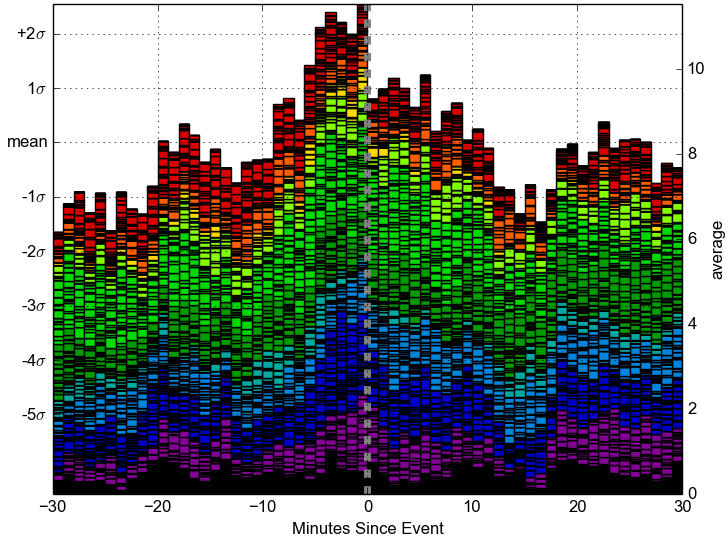
\includegraphics[width=0.9\columnwidth]{./img/mAvatarViews_586_noOverlap.png}
\caption{Stackplot of step counts in the 30 minutes surrounding 586 phone-view events from the mAvatar dataset with no other events within 30min.}
\label{fig:mAvatarNoOverlap}
\end{figure}

Event overlap becomes somewhat inevitable, however, for large event window sizes.
Figure \ref{fig:mAvatarNoOverlap} shows a selection of data identical to that in figure \ref{fig:mAvatarPhoneContext}, but without the inclusion of overlapping windows of analysis surrounding the events.
Allowing no overlap between events helps ensure that multiple interventions effects do not skew the data, but ignoring these data points can drastically reduce the sample if large times following the event are used, because very few events are so isolated.

\begin{figure}
\centering
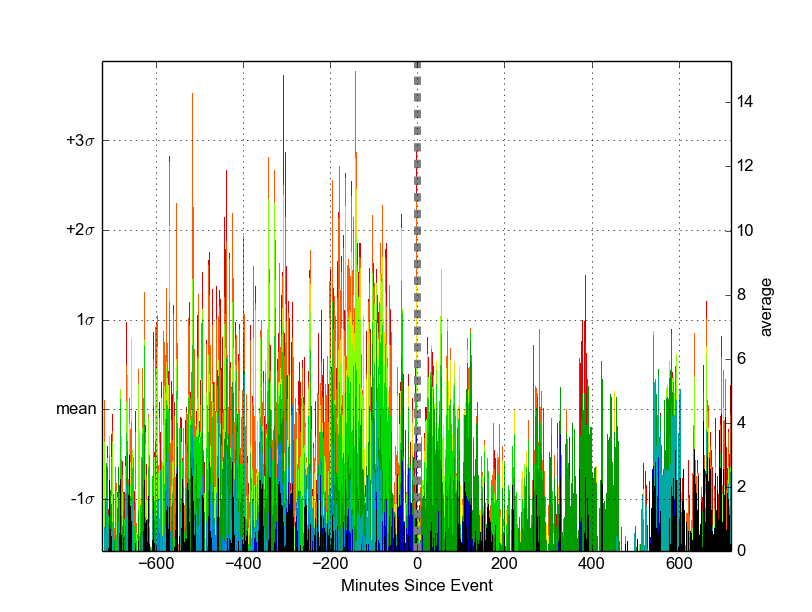
\includegraphics[width=0.9\columnwidth]{./img/mAvatarViews_46_12hr_noOverlap.png}
\caption{Stackplot of step counts in the 12hrs surrounding 46 phone-view events from the mAvatar dataset with no other events within 12 hours.}
\label{fig:mAvatarNoOverlap12hr}
\end{figure}

As is shown in \ref{fig:mAvatarNoOverlap12hr}, increasing the window of analysis to 12hours surrounding the phone-view event leaves only 46 events, and a noticeable increase in the variability of the data is observed.

\begin{figure}
\centering
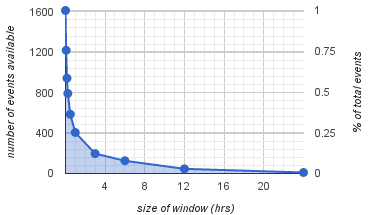
\includegraphics[width=0.9\columnwidth]{./img/events_v_windowSize.png}
\caption{Percent coverage of events in the mAvatar datset vs size of exclusion window surrounding the event.}
\label{fig:eventsVwindow}
\end{figure}

For phone-view events among the population analyzed by the mAvatar study, we can estimate percent coverage of events available for ``clean'', non-overlapping analysis through the distribution shown in figure \ref{fig:eventsVwindow}.

\subsection{Alternative Stacked-Area Representation}
Use of the "themeRiver/streamgraph" \cite{havre2000, byron2008} paradigm for plotting stacked area charts may offer an improved view of the contribution of individual time series to the aggregated result, further easing the identification of outlier participants or events.

With better focus on individuals or subgroups, however, comes a reduced ability to look at the bigger picture.
Thus, although a streamgraph may make for a better general view, the stacked area plots presented are still of use for those whose primary focus it is to evaluate the group response.

\comment{ things covered by this section are well discussed elsewhere
  \subsection{Modeling Observed Effects}
  Ever since [], behavioral scientists have sought theories to explain, influence and change human behavior.


  TODO? Some example models of the aforementioned effects for control and/or KNOWME data.

  transfer function modeling?
  fitting of a fluid-flow analogy using a priori constructs?
  other?
}

\subsection{Characterizing Psychological Influence of Events via Response Signature}
Different psychological mechanisms act on different time-scales and, likewise, with different dynamics. 
The delay of effect onset and decay of the effect observed in data could theoretically be used to suggest what psychological mechanisms are at work.
In this way, interventions could be characterized in terms of applicable theory via the the dynamics observed.

This method becomes even more powerful when responses across multiple variables are considered.
To draw an example from previously presented data, a combined analysis of heart rate (figure 1C) and accelerometer count (figure \ref{fig:knowMeCompare}) dynamics improves the ability to match signals to known responses.

\subsection{Statistical Analysis of Features}
Much existing work on the statistical testing of between-phase differences in traditional AB study designs \cite{parker2003} is applied in the evaluation of the efficacy of a one-time or repeatedly applied intervention, and methods for evaluating the likelihood of features in a time-series are also well documented \cite{gorman1996, suen1989}.
Through combination of existing intervention analysis techniques \cite{box1975}, goodness-of-fit evaluations of model formulations \cite{pankratz2012} in comparison to surrogate time series, and the presented visualization methods, researchers have a good foundation for analyzing dynamic models of human behaviors. % to enable clever JiTAIs.
